\documentclass{beamer}

\usetheme{Rochester}
\usefonttheme{default}
\usecolortheme{whale}

\newcommand{\kcolor}[1]{\lceil \sqrt{\log{#1}} \rceil}

\title[Graph Minors and the Robertson-Seymour Theorem]{\small{Presentation On} \\ \Large{Graph Minors and the Robertson-Seymour Theorem}}
\subtitle{Parameterized Algorithms, Springer}

\author[1705066]{\small{1705066 - Ataf Fazledin Ahamed}}

\date{\today}

\institute[BUET]{Bangladesh University of Engineering and Technology}

\begin{document}

\maketitle

\begin{frame}{Outline}
    \tableofcontents
\end{frame}

\section{Introduction}

\begin{frame}{Introduction}
    \only<1>{
        We discuss the minor relation in graphs and the algorithmic usage of the \alert{Robertson-Seymour Theorem}
    }
    \only<2>{
         \begin{block}{Robertson-Seymour Theorem}
            \begin{enumerate}
                \item {by Neil Robertson and Paul D. Seymour}
            \end{enumerate}
         \end{block}
    }
    \only<3>{
         \begin{block}{Robertson-Seymour Theorem}
            \begin{enumerate}
                \item {by Neil Robertson and Paul D. Seymour}
                \item {proved in a series of 20 papers}
            \end{enumerate}
         \end{block}
    }
    \only<4>{
         \begin{block}{Robertson-Seymour Theorem}
            \begin{enumerate}
                \item {by Neil Robertson and Paul D. Seymour}
                \item {proved in a series of 20 papers}
                \item {spanning over 500 pages}
            \end{enumerate}
         \end{block}
    }
   \only<5>{
         \begin{block}{Robertson-Seymour Theorem}
            \begin{enumerate}
                \item {by Neil Robertson and Paul D. Seymour}
                \item {proved in a series of 20 papers}
                \item {spanning over 500 pages}
                \item {from 1983 to 2004}
            \end{enumerate}
         \end{block}
    }
    \only<6>{
        No, we are not going to prove it today.
    }
\end{frame}

\section{Graph Minors}
\begin{frame}{Graph Minors}
    \only<1,2,3>{A graph \textit{H} is a minor of graph \textit{G}, denoted by \textit{H} \leq _{m} \textit{G},}
    
    \only<2,3>{if \textit{H} can be obtained from some \alert{subgraph} of \textit{G} by a series of edge contractions.}

    \only<3>{
        \vspace{0.2in}
        Equivalently, graph \textit{H} is a minor of \textit{G}, if \textit{H} can be obtained from \alert{\textit{G} itself} by a series of edge deletions, edge contractions, and vertex deletions.
    }

    \only<4>{
        \begin{figure}
            \centering
            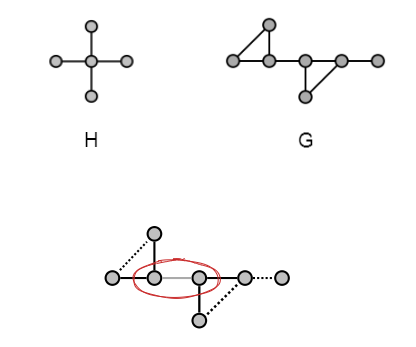
\includegraphics[height = 0.6\textheight]{img/0.PNG}
            \caption{Graph H is a minor of graph G}
        \end{figure}
    }

    \only<5>{
        The theory of graph minors began with Wagner's Theorem - that a graph is planar if and only if its minor include neither the complete graph {\textit{K}_{5}} \\  nor the complete bipartite graph \textit{K}_{3,3} \\
    } 

    \only<6>{
        \begin{block}{Forbidden Graph Minors}
            A forbidden graph minor is a method of specifying a family of graph by specifying minors that are forbidden from existing within any graph in the family.
        \end{block}
    }

    \only<7>{
        \begin{block}{Graph Minors Properties}
            A number of interesting properties of graphs are preserved under deletions and edge contractions can be characterized by forbidden minors.
            \\
            \\
            \textit{Example: Planarity, Coloring, etc.}
        \end{block}
    }

    \only<8>{
        Few observations:
        \\
        \\
        A graph is a forest if and only if it has no minor isomorphic to the triangle \alert{$K_3$}. (Proof is trivial.)
        \begin{figure}
            \centering
            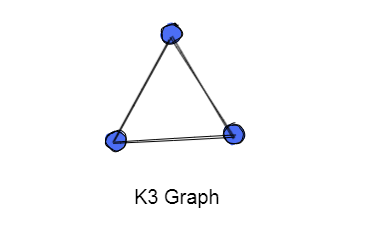
\includegraphics[height = 0.4\textheight]{img/1.PNG}
            \caption{Graph $K_3$}
        \end{figure}
    }

    \only<9>{
        \vspace{0.1in}
        A graph is planar if and only if it has no minor isomorphic to \alert{$K_{5}$ or $K_{3,3}$}. This is Wagner’s theorem.
        \begin{figure}
            \centering
            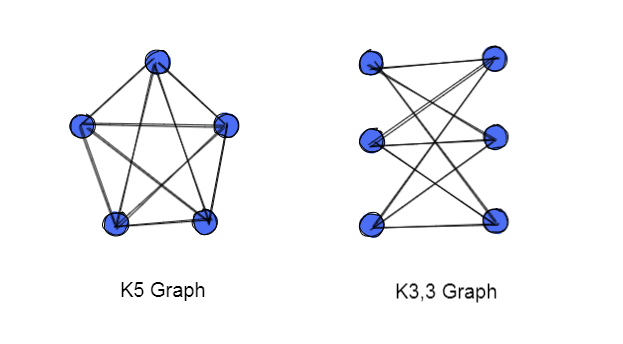
\includegraphics[height = 0.4\textheight]{img/2.PNG}
            \caption{Graph $K_{5}$ and $K_{3,3}$}
        \end{figure}
    }

    \only<10>{
        \vspace{0.1in}
        A graph is outerplanar if and only if it has no minor isomorphic to \alert{$K_{4}$ or $K_{2,3}$}.
        \begin{figure}
            \centering
            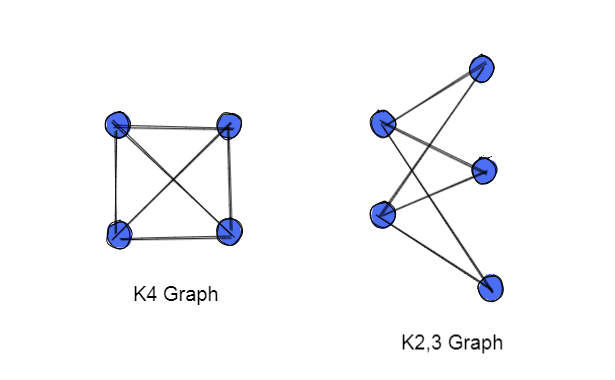
\includegraphics[height = 0.4\textheight]{img/3.PNG}
            \caption{Graph $K_{4}$ and $K_{2,3}$}
        \end{figure}
    }
\end{frame}

\section{Few Observations}
\begin{frame}{Few Observations}
    \only<1>{
        \begin{block}{Proposition 6.8}
            A minor of a planar graph is also planar.
        \end{block}
        \vspace{0.15in}
        \begin{quote}
            Removing edges and vertices cannot make a planar graph non-planar. It is the other way round.
        \end{quote}
    }

    \only<2>{
        \begin{enumerate}
            \item{
                It is known that a graph can be drawn on a plane if and only if it can be drawn on a sphere.
            }
            \item{
                However, there are graphs that can only be drawn on a torus, but not on an sphere. For example- the $K_{5}$ graph.
            }
            \item{
                Similar cases exist for weird surfaces, such as- Klein Bottle, The Projective Plane, etc.
            }
        \end{enumerate}
    }

    \only<3>{
        \begin{block}{Statement}
            If a graph G is embeddable in a surface $\Sigma$, and H is a minor of G, then, H is also embeddable on $\Sigma$ as well.
        \end{block}
        \vspace{0.15in}
        \begin{quote}
            Such observations and findings have applications in \\
            Topological Graph Theory.           
        \end{quote}
    }
    
\end{frame}

\section{The Robertson-Seymour Theorem}

\begin{frame}{Robertson-Seymour Theorem: Few Terminologies}
    \only<1>{
        \begin{block}{Quasi-ordering or Pre-ordering}
            A pre-order or quasi-order of a set is a binary relation among its elements that is both reflexive and transitive.
        \end{block}
    }    
    \only<2>{
        \begin{block}{Quasi-ordering or Pre-ordering}
            Consider a relation $\leq$ on a given set P, so that $\leq$ is a subset of $P x P$ and notation $ a \leq b$ is used in place of $(a, b) \in \leq $. Then $\leq$ is called a pre-order or quasi-order if it is both reflexive and transitive.

            \vspace{0.1in}
            \textbf{Reflexivity:} $ a \leq a $ for all $ a \in P $ and
            \\
            \textbf{Transitivity:} $ a \leq b $ and $ b \leq c $ then $ a \leq c $ for all $ a, b, c \in P $
        \end{block}
    }
    \only<3>{
        \begin{block}{Well-Quasi-Ordering}
            A well-quasi-ordering or wqo is a quasi-ordering such that any infinite sequence of elements $ x_{0}, x_{1}, x_{2}, ... $ from $ X $ contains an increasing pair $ x_{i} \leq x_{j} $ with $ i < j $
        \end{block}    
    }
\end{frame}

\begin{frame}{Robertson-Seymour Theorem}
    \begin{block}{Theorem 6.10 (Robertson and Seymour)}
        The class of all graphs is \textbf{well-quasi-ordered} by the minor relation. That is, in any infinite family of graphs, there are two graphs such that one is a minor of the other.
    \end{block}
\end{frame}

\begin{frame}{Application}
    \only<1>{
        $\textit{Forb} ( \mathcal{G} ) \leftarrow $ Family of minimal forbidden minors for $ \mathcal{G} $
    }

    \only<2>{
        \begin{block}{Corollary 6.11}
            For every minor-closed graph class $ \mathcal{G} $, there exists a finite set   $ \textit{Forb}(\mathcal{G}) $ of graphs with the following property: for every graph G, graph $ G \in \mathcal{G} $ if and only if there does not exist a minor of G isomorphic to a member of $\textit{Forb} ( \mathcal{G} ) $.
        \end{block}
    }

    \only<3,4>{
        Corollary 6.11 and Theorem 6.10 gives us the following:
        \vspace{0.1in}

        \begin{block}{Theorem 6.12 (Robertson and Seymour)}
            There exists a computable function \mathcal{f} and an algorithm that, for every given graphs \textit{H} and \textit{G}, checks in time $ f(H)|V(G)|^3 $ whether $ H \leq _{m} G $
        \end{block}
    }
    \only<4>{    
        Which implies that every minor-closed class can be recognized in polynomial time.
    }
\end{frame}


\section*{}
% Q&A
\begin{frame}
    Thank You
\end{frame}
\end{document}
